\section{Problem formulation}
\label{sec:ftp}

Consider a tourist who wishes to take a trip that visits every node (city) $i$
in the set of nodes $V$, $|V|$ = $N$, with no particular order. The start node
will be denoted as $v_{0}$, while the return node as $v_{n+1}$, and the complete
set of nodes is given by $V_c$ = $V \cup \{v_0\} \cup \{v_{n+1}\}$. The trip
must start at a time $t \in T_0 = [T_{0m}, T_{0M}]$. Upon visiting a node, the
tourist will stay there for a duration of $d$ time-units (days). Consider that
for each node to be visited, there is a range for the value $d$ might take, that
  d_i \in [d_{im}, d_{iM}]$ and $d_{iM} \geq d_{im} \geq 1$ (nights). The complete
set of durations associated to each city is given by D, and $|D| = N$.
Furthermore, to each city $i \in V$, there is an associated time-window $TW$,
$|TW| = |V| = N$, which defines the set of dates in which the city $i$ may be
visited.

By following this definition, the FTP is completely defined by a structure $G =
(V_c, A, T_{0}, D, TW)$, used to create a multipartite graph describing the
request. This multipartite graph is divided into $k$ layers, where each layer
corresponds to a particular moment in time. Besides this, every node in a layer
is connected to all nodes in the subsequent layer. The set of arcs that connects
these nodes is given by $A$. To each arc $a \in A$, it is associated a cost
$c_{a}$ (ticket cost) and a processing time $p_{a}$ (flight duration), which
depend upon the routed nodes, as well as the time in which the arc transition is
initiated, that is, $\forall a_{ij}^{t} \in A$, $c_{ij}^{t} \geq 0$ and
$p_{ij}^{t} \geq 0$.

A valid solution $s$ to the FTP is a set of arcs (commercial flights)
which start from node $v_0$ during the defined start period, visit every node
$i$ in $V$ during its defined time-window $TW(i)$, and respect the duration of stay in each node, defined by $D(i)$, before finally returning to node $v_{n+1}$. The set of
all valid solutions is given by $S$. The goal of the FTP is to find the global
minimum $s^* \in S$, with respect to the considered objective function.

The objective function associated to this problem depends on the user criteria.
While some users might consider the total cost to be the most important
factor, others may consider that the total flight duration is of crucial
importance. Thus, a total of three different objective functions shall be herein
considered: (i) the expended cost (see eq. ~\ref{eq:obj_cost}), (ii) the flight
duration (see eq.~\ref{eq:obj_time}), and (iii) the resulting entropy (see
eq.~\ref{eq:obj_entropy}), where the latter corresponds to a weighted sum
between the former two. 
\begin{equation}
\label{eq:obj_cost}
  F_{c}(s) = \sum_{n=0}^{N+1} c(s[n])
\end{equation}

\begin{equation}
\label{eq:obj_time}
  F_{t}(s) = \sum_{n=0}^{N+1} p(s[n])
\end{equation}

\begin{equation}
\label{eq:obj_entropy}
  F_{e}(s) = \sum_{n=0}^{N+1} w_c*c(s[n]) + w_p*p(s[n])
\end{equation}

Figure \ref{fig:multipartite_sol} illustrates the multipartite graph associated
to a simple instance of the FTP with $v_{n+1} = v_0 = X$, one possible start
date ($t = 0$), 3 nodes to visit $(A, B, C)$, with a fixed duration of
respectively (1,2,3) time-units, and no constraints relative to the time-window
of each city. A possible solution to this problem instance corresponds to the
set of arcs $(a_{X,B}^{0}, a_{B,A}^{2}, a_{A,C}^{3}, a_{C,X}^{6})$.

\begin{figure}[tbp]
  \centering
  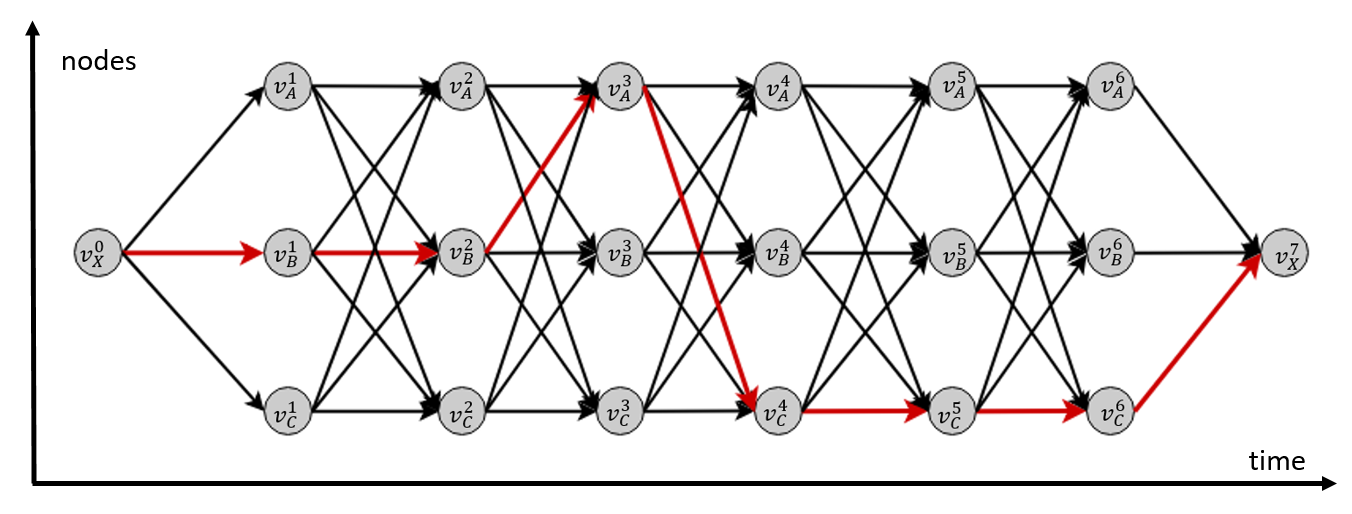
\includegraphics[width=1.0\columnwidth]{./imgs/multipartite_axis.png}
  \caption{Illustration of a Flying Tourist Problem using a multipartite graph. To each node (A,B,C) it is associated a waiting period of respectively (1,2,3) time units. The red arrows represent a possible solution to the problem.}
  \label{fig:multipartite_sol}  
\end{figure}


Despite the apparent complexity of the proposed definition, it can be used to
state very simple flight searches, including one-way and round-trip flights. For
example, the problem of finding a single flight from $A$ to $B$ at date $T$ can
be instantiated as a FTP given by $v_0$ = $A$, $v_{n+1}$ = $B$, $T_{0} = T$, and
$V$ = $D$ = $TW$ = $\{\}$. In its turn, a round-trip flight involving the same
two cities and the same start date, in which the staying period in $B$ is $b$
days, is given by $v_0 = v_{n+1} = A$, $T_{0} = X$, $V = \{B\}$, $D = \{b\}$ and
$TW$ = $\{\}$. Thus, this definition is adequate either for simple and complex
trips, which can be customized according to the user search criteria, by setting
either an extended start dates, or flexible durations.